\subsection*{Introduction to Communication Systems}

\setlength{\intextsep}{0pt}
\begin{figure}[H]
    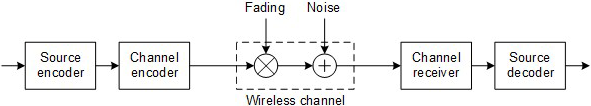
\includegraphics[width=\linewidth]{images/wireless_channel_model.png}
\end{figure}
\textbf{Source encoder:}

Réduit la quantité de données à transmettre ou à stocker, tout en préservant la qualité de
l'information.
Deux types de codage de source, selon que l'on accepte ou non une
perte d'information:

\underline{Lossless coding}: permet de reconstruire exactement les données d'origine à
partir des données codées. Exemples : codage de Huffman, codage arithmétique, codage Lempel-Ziv.

\underline{Lossy coding}: introduit une dégradation irréversible de l'information, mais permet
d'obtenir des taux de compression plus élevés. Exemples : codage par transformée,
codage par quantification vectorielle, codage par prédiction linéaire.

Deux critères pour évaluer la performance d'un codage de source:

\underline{Taux de compression}: rapport entre la quantité de données d'origine et la
quantité de données codées. Plus il est élevé, plus le codage est efficace.

\underline{Distorsion}: mesure de la différence entre les données d'origine et les données
reconstruites. Plus elle est faible, plus le codage est fidèle.

\textbf{Channel encoder:}

Permet de protéger les données contre les erreurs de transmission en ajoutant de la redondance.
Deux types principaux de codage de canal:

\underline{Codage en bloc}: Consiste à diviser les données en blocs de taille fixe et à ajouter
des bits de parité pour détecter et corriger les erreurs.

\underline{Codage Convolutif}: Consiste à appliquer une fonction de transfert aux données en
tenant compte des bits précédents et à générer des bits de contrôle pour détecter et
corriger les erreurs.

\textbf{Wireless channel:}

Support physique qui permet de transmettre les signaux entre l'émetteur et le récepteur.
Il peut être filaire (câble coaxial, fibre optique, etc.) ou sans fil (ondes radio, infrarouge,
etc\dots). Le canal de communication est caractérisé par sa bande passante, qui est la gamme
de fréquences qu'il peut transmettre, et son atténuation, qui est la diminution de l'amplitude
des signaux au cours de la propagation.

Il est imparfait et introduit des perturbations qui altèrent les signaux transmis :

\underline{Bruit}: Variation aléatoire du signal.

\underline{Distorsion}: Modification de la forme du signal.

\underline{Interférence}: Superposition de signaux indésirables.

Les perturbations peuvent entraîner des erreurs de transmission, c'est-à-dire des différences
entre le signal émis et le signal reçu. Pour limiter les erreurs de transmission,
on utilise des techniques de codage, qui consistent à ajouter de l'information redondante
au signal, et de modulation, qui consistent à adapter le signal à la bande passante du canal.
